\documentclass[]{article}
\usepackage[margin=1in]{geometry}
\usepackage{graphicx}
\usepackage{lscape}
\usepackage{mathtools}
\usepackage{listings}
\lstset{ %
language=Java,                % choose the language of the code
}
\begin{document}

\title{SmokeSNET Model}
\author{Matt Smith}
\date{\today}
\maketitle

\section{Current Attributes}

\begin{table}
    \begin{tabular}{|l|l|p{12cm}|}
        \hline
        Name & Type & Represents \\ \hline
        	isSmoker &  Boolean & True if they're a smoker, false otherwise \\ 
 	willpower &  Double & A probability representing willpower, 0 being of strong willpower. \\ 
	health &  Double & A value between 0 and 1 for health, where 1 is perfect health and 0 is a smoking-related disease.\\ 
	smokedPerDay &  Integer & The number of cigarettes smoked per day\\ 
	givingUp & Boolean & A side-status for non-smokers, where true means they are giving up. Every turn this can influence whether a person starts again, whether they become a \'normal\' non-smoker and can affect others who are also giving up. \\ 
 	giveUpAttempts & Integer & The number of attempts at giving up. \\ 
 	stepsSinceGiveUp &  Integer & The number of simulation steps since the last decision to give up. \\ 
	sociable &  Double & A probability representing how sociable someone is, with 1 being very sociable \\ 
        \hline
    \end{tabular}
\label{attr}
\caption{Model Attributes}
\end{table}
As it stands, nodes have the attributes seen in figure \ref{attr}.
Edges are directed and their weight is a probability, representing their influence.
Currently, all attributes are normally distributed and can be adjusted to more realistic values later in development.
Nodes can also be constrained to a maximum number of in-edges, i.e. nodes which influence them. Within each simulation step, the following happens:
\begin{enumerate}
\item The local neighbourhood within three incoming hops is acquired for the given node. Influence between the nodes is calculated as the maximum influence across all possible connections of the two nodes, where influence over multiple hops is the product of the influence of each hop. For example, in Fig. \ref{networkdiag}, the influence of \emph{Node C} on the \emph{Current Node} is the maxiumum of $0.8 * 0.8$ and $0.1$, where the best value here is $0.64$ for \emph{Node C} to \emph{D} to \emph{Current}. Note that even if a one-hop route exists, the maximum influence will be chosen for consistency across the neighbourhood. All nodes within the neighbourhood set are unique.
\begin{figure}
\begin{center}
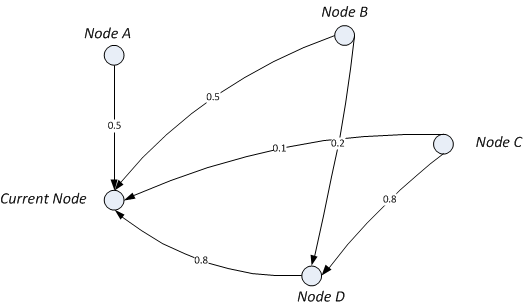
\includegraphics{networkdiag.png}
\label{networkdiag}
\caption{Network Diagram}
\end{center}
\end{figure}

\item Metrics for this set are calculated for the current node relative to the neighborhood. Some general ones, such as the percentage of the neighbourhood which is giving up smoking, along with the percentage that currently smoke is calculated. For each node attribute, the influence weighted average seen in figure \ref{inf} is calculated.
\begin{figure}
	\begin{center}
		\begin{math}
		\frac{\sum_{\forall n \in N} attribute_{n} \times influence_{n}}{\sum_{\forall n \in N} influence_{n}} \text{ where } N \text{ is the set of nodes}
		\end{math}
	\end{center}
	\label{inf}
	\caption{Influence Calculation}
\end{figure}


\item The decision tree is run on the nodes. At present, this tree can be drawn as seen in figure \ref{dectree}. The relevant probability calculations are in figure \ref{decTreeProbs}. For decisions such as `Is a Smoker?', the decision is based on the attribute value so no probability needs to be calculated. For each, a random number between $0$ and $1$ is generated - if it is lower than the calculated probability, then the decision is considered to have happened. The aim of the decision tree is to adjust the attribute values of the individual node. 
\begin{figure}
\begin{center}
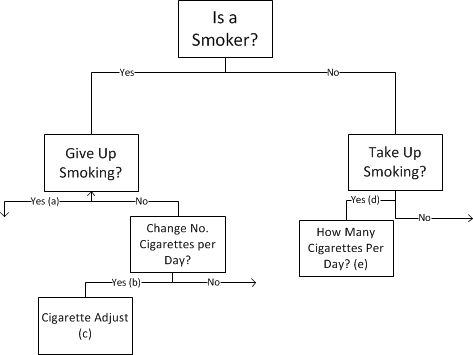
\includegraphics{DecTreeBasic2.png}
\label{dectree}
\caption{Decision Tree}
\end{center}
\end{figure}


\begin{figure}
	$\forall n \in Nodes$

	\begin{enumerate}
		\item p(give up smoking)=$(1-health_{n}) \times \frac{|\text{Nodes giving up smoking}|}{|\text{Nodes}|}$ \\
		\item If $n$ smokes $\pm10\%$ of the influence sum for cigarettes smoked, and $n$\'s health is within $\pm10\%$ of the influence sum of health. \\
		\item $change = (\text{influence sum of smoked per day} - {smokedPerDay}_{n}) \times influenceability_{n}$, else there is no change. \\
		\item p(take up smoking) = $health_{n} \times \frac{|\text{Nodes giving up smoking}|}{|\text{Nodes}|} \times \frac{|\text{Nodes who smoke}|}{|\text{Nodes}|}$ \\
		\item If the influenced sum of the number of cigarettes per day is $< 0$, then $smokedPerDay = 5$, otherwise \\
		$smokedPerDay = \operatorname{round}(\frac{\sum_{\forall n \in Neighbours} smokedPerDay_{n} \times influence_{n}}{\sum_{\forall n \in N} influence_{n}})$
	\end{enumerate}
	\label{decTreeProbs}
	\caption{Decision Tree Calculations}
\end{figure}

\item Finally, a nodes connections are adjusted based on its attributes. Currently, the nodes have an upper limit of in-edges, representing influence on the node - (simulations run with 10 at the moment) to avoid hugely saturating the graph. If a node reaches this maximum but still wishes to add an edge, it can remove a low influence edge $e$ with a probability $p(removal) = (1 - \operatorname{min}_{\forall e \in \text{In Edges}}(influence_{e}))$.
\\
Edges are selected for addition based on a scoring system of each node in the \emph{n}-hop neighbourhood. The system uses multiple approaches to determine a score (i.e. a 'worthiness') for each of these nodes:
\begin{enumerate}
\item Boolean scoring, where the node either gets all the points, or none of the points
\item Linear scoring, in which the percentage difference of the node being considered from the source node is deducted from a points total, i.e. $score = maxPoints - \text{\% diff} \times maxPoints$ - if the target node is $100\%$ or over different, then they will score zero on that comparison.
\item Range scoring, where if one node is within a given range of another, a set score is given.
\item Percent scoring, where the attribute is multiplied against a maximum score to get the net score. 
\end{enumerate}
The current scoring algorithm can be seen in figure \ref{pseudo}. It is very basic and as such, gives little spread in the scores of nodes. The effect of this is that it becomes difficult to differentiate good connection candidates from average or poor ones - a way to circumvent this is to add in extra attributes and tune the scores per attribute until a reasonable spread is given.

\begin{figure}
\begin{center}
	\begin{lstlisting}
for(Node n : Neighbours)
{
	if(current.isSmoker == n.isSmoker)
	{
		score + 1
		if(current.isGivingUp && n.isGivingUp)
		{
			score + 2
			if(n.stepsSinceGiveUp is within 50% of current.stepsSinceGiveUp)
				score + 5
			else
				score + 2
		}
		if(current.isSmoker)
		{
			score + linearScore(smokedPerDay) 	//Max 5 pts
		}
	}
	score + linearScore(health)		//Max 5 pts
	score + linearScore(willpower)		//Max 5 pts
	score + linearScore(sociable)		//Max 5 pts

	score + percentScore(influenceability)	//Max 5 pts
	score + percentScore(persuasiveness)	//Max 5 pts

	return score/33
}
	\end{lstlisting}
\end{center}
\label{pseudo}
\caption{Scoring Algorithm}
\end{figure}
The total score is divided by the maximum available score to give a value between $0$ and $1$. A threshold is then set to determine whether to add or remove the edge (i.e. if the score is less than $0.1$, remove the edge, if it is between $0.1$ and $0.2$ do nothing, otherwise add it.

\end{enumerate}
\section{Upcoming Features}
\begin{itemize}
\item A more complex decision tree, incorporating all attributes and causing gradual change over time.
\item Network metric analysis during the simulation to check if the graph is converging to a `small world' style graph. This is through looking at the average clustering coefficient of the graph, and depending on the results of this, further graph statistics.
\item More attributes that affect smoking cessation being added.
\end{itemize}

\end{document}